%%%%%%%%%%%%%%%%%%%%%%%%%%%%%%%%%%%%%%%%%%%%%%%%%%%%%%%%%%%%%%%%%%%%%%%%%%%%%%%%
%2345678901234567890123456789012345678901234567890123456789012345678901234567890
%        1         2         3         4         5         6         7         8

\documentclass[letterpaper, 10 pt, conference]{ieeeconf}  % Comment this line out if you need a4paper

%\documentclass[a4paper, 10pt, conference]{ieeeconf}      % Use this line for a4 paper

\IEEEoverridecommandlockouts                              % This command is only needed if 
                                                          % you want to use the \thanks command

\overrideIEEEmargins                                      % Needed to meet printer requirements.

% See the \addtolength command later in the file to balance the column lengths
% on the last page of the document

% The following packages can be found on http:\\www.ctan.org
%\usepackage{graphics} % for pdf, bitmapped graphics files
%\usepackage{epsfig} % for postscript graphics files
%\usepackage{mathptmx} % assumes new font selection scheme installed
%\usepackage{times} % assumes new font selection scheme installed
%\usepackage{amsmath} % assumes amsmath package installed
%\usepackage{amssymb}  % assumes amsmath package installed
\usepackage{graphicx}
\usepackage[export]{adjustbox}
\graphicspath{ {images/} }


\title{\LARGE \bf
Traversibility Ground Truth for Planning :\protect\\
DNN Training in Simulation
}


\author{ % <-this % stops a space
\thanks{This work was supported by the Robotics Master Program in National Chiao Tung University, Taiwan}% <-this % stops a space
\thanks{Thanks Lily Hsu and Michael Tsai, our best team}%  
}


\begin{document}



\maketitle
\thispagestyle{empty}
\pagestyle{empty}


\section{INTRODUCTION \& MOTIVATION}
In the complex man-made environment, it's very hard for someone impaired to walk around and interact with surroundings. Likewise, it's a difficulty for a robot with  finite sensor and  incomplete cognition to traverse around. It's a critical problem for the upcoming robotics era, we must make sure the robot will not be damaged doing their task, especially for movable robot. It's an important issue to help others impaired to have more freedom in movability. We try to mimic the two problem  into the planning solution in autonomous mobile robots. There are servel research about planning in terrain, terrain classification and traversability algorithm in past years, we try to combine some approach in previous research with our simulation platform and algorithm to bring the effect in 
the problem planning in terrain or terrain modeling. 


For terrain modeling or terrain definition, A. Chilian and H. Hirschm ̈uller \cite{chilian2009stereo} uses a depth information and pose estimation to create DEM(digital elevation model) of the surrounding and give properties of terrain using roughness, slope and step height. R. O. Chavez-Garcia, J. Guzzi, L. M. Gambardella, and A. Giusti\cite{chavez2017learning} create terrain by synthesizing real heightmap data and maunal terrains using procedural generation techniques in Gazebo and similar ways is done in\cite{hewitt2017training}, both two highly depends on simulation modeling, which are similar with our approach.  For travesibility, there are ways of defining travesibility with robot model and pose \cite{zimmermann2014adaptive} \cite{dupont2008terrain}, K. Zimmermann, P. Zuzanek, M. Reinstein, and V. Hlavac \cite{zimmermann2014adaptive} gives a discrete way to define robot motion, which is more adative for different robot. In the last training part, there are many different training algorithm 
to define travesibility by learning, and almost all of the reference paper\cite{chavez2017learning}\cite{hewitt2017training}\cite{zimmermann2014adaptive}\cite{dupont2008terrain}\cite{kim2007traversability}\cite{kim2006traversability}are using training way to give the travesibility.


\begin{figure}[t] % h means put this image here
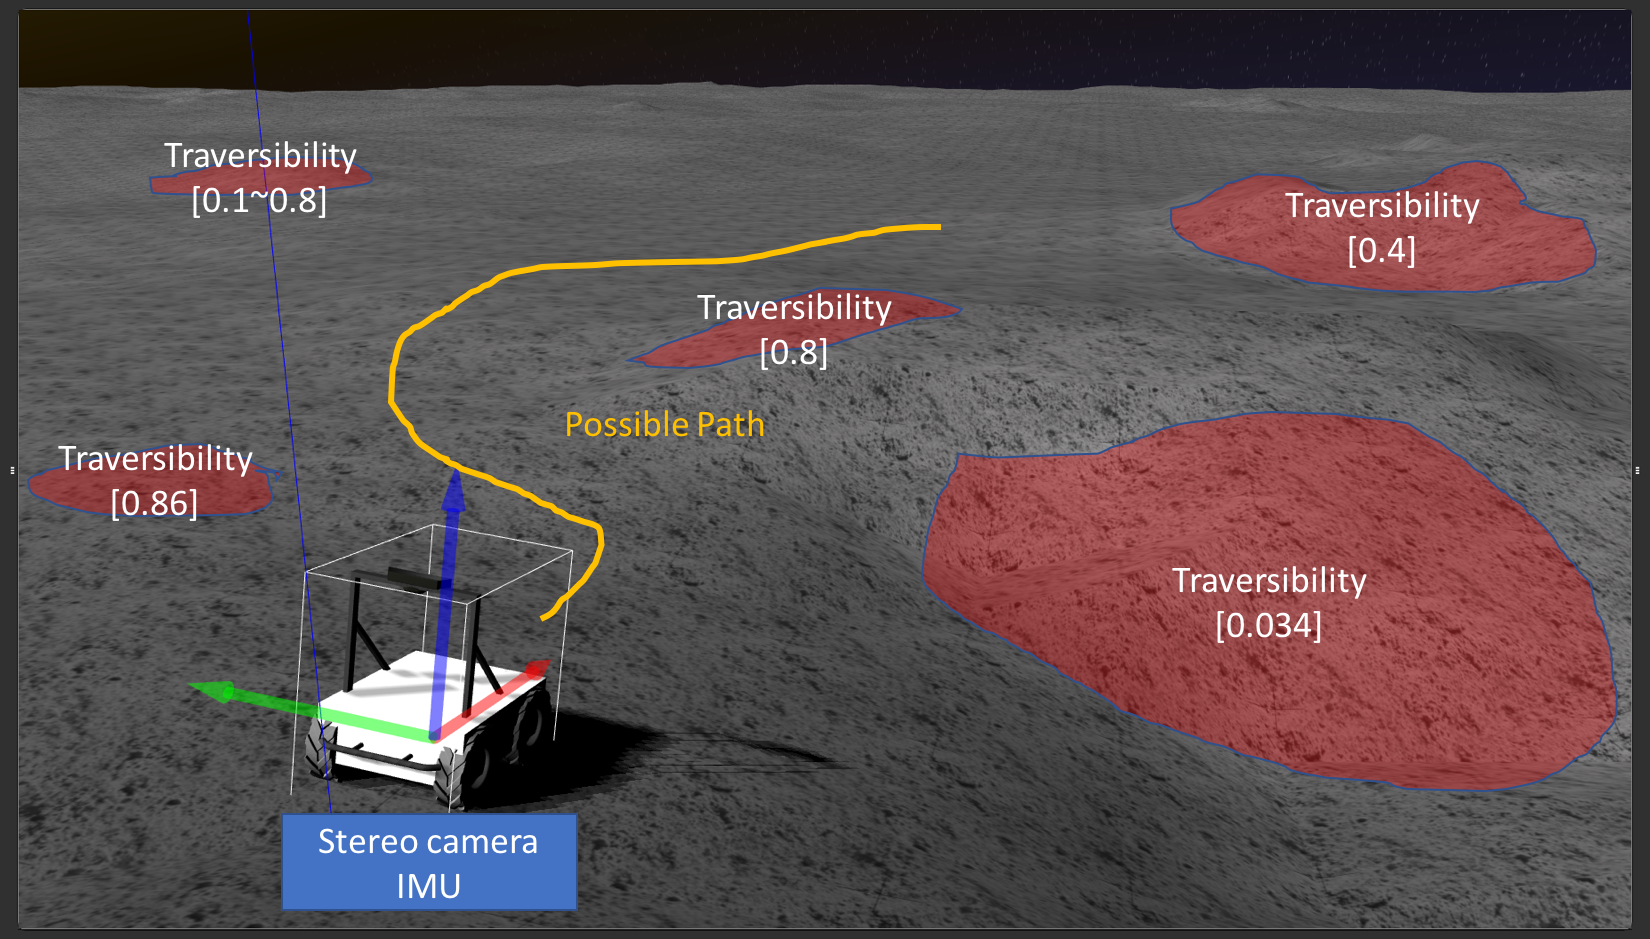
\includegraphics[width=0.8\columnwidth]{teaser}
\centering
\caption{Planning in Terrain}
 \label{figure:teaser}
\end{figure}


In this proposal we propose to use a pre-trained model using CNN,whcih is similiar with \cite{chavez2017learning}, with high dimensional inputs from the visual sensor real-sense and  IMU (inertial measurement unit), enabling the robot to sense its terrain by feeling and seeing , similar to how humans determine the terrain on which they are driving,  to traverse an  unknown outdoor environment and  reach the designated goal without human intervention. A key aspect of this task is to determine the traversability of the outdoor terrain, we use \cite{JiatongBao2012} simple way to calculate traversability. And we try to get the ground truth of  fixed-size patches in the depth image. After knowing every patches ground truth in the depth image, then we apply planning algorithm. 
\section{SYSTEM ARCHITECTURE \& EQUIPMENTS}

\subsection{SYSTEM ARCHITECTURE}

There are two parts in our system, training part and prediction part Fig.2 and Fig.3. In prediction part , we use Gazebo to simulate our robot and terrain, which the robot is modifying from the Husky with 30x30x12 cm3 big tires equipped with stereo camera and IMU. The stereo camera is about 20 degrees looking to the ground and the IMU is simulating with a box, putting in the centroid of our robot. The sensor data will using some mixture to generate a high-dimensional input which is the input of the DNN training model.
After the training part, we will put the training model on  the robot, to get the ground truth from the real-time depth image, and apply planning algorithm.

\subsection{EQUIPMENTS} 
Since we are using simulation, there is no any hardware.  
\begin{figure}[h] % h means put this image here
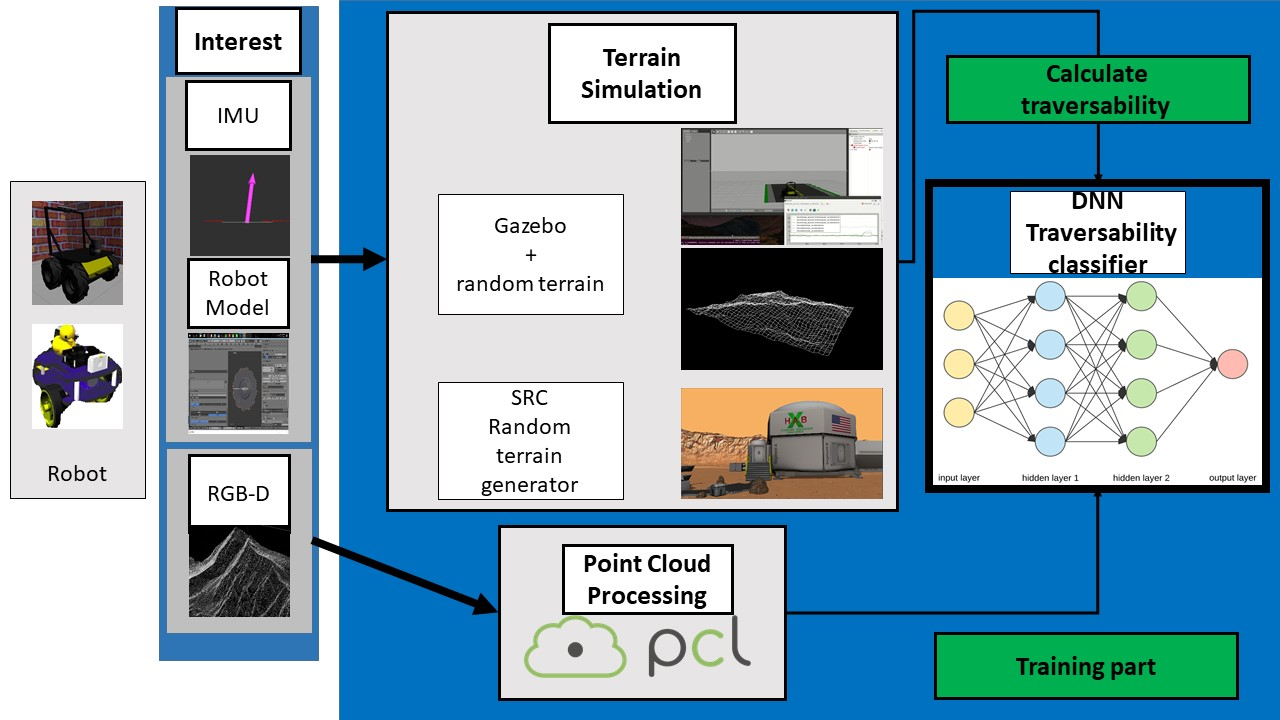
\includegraphics[width=0.8\columnwidth]{sys1}
\centering
\caption{Training}
 \label{figure:training}
\end{figure}

\begin{figure}[t] % t means put this image at the top 
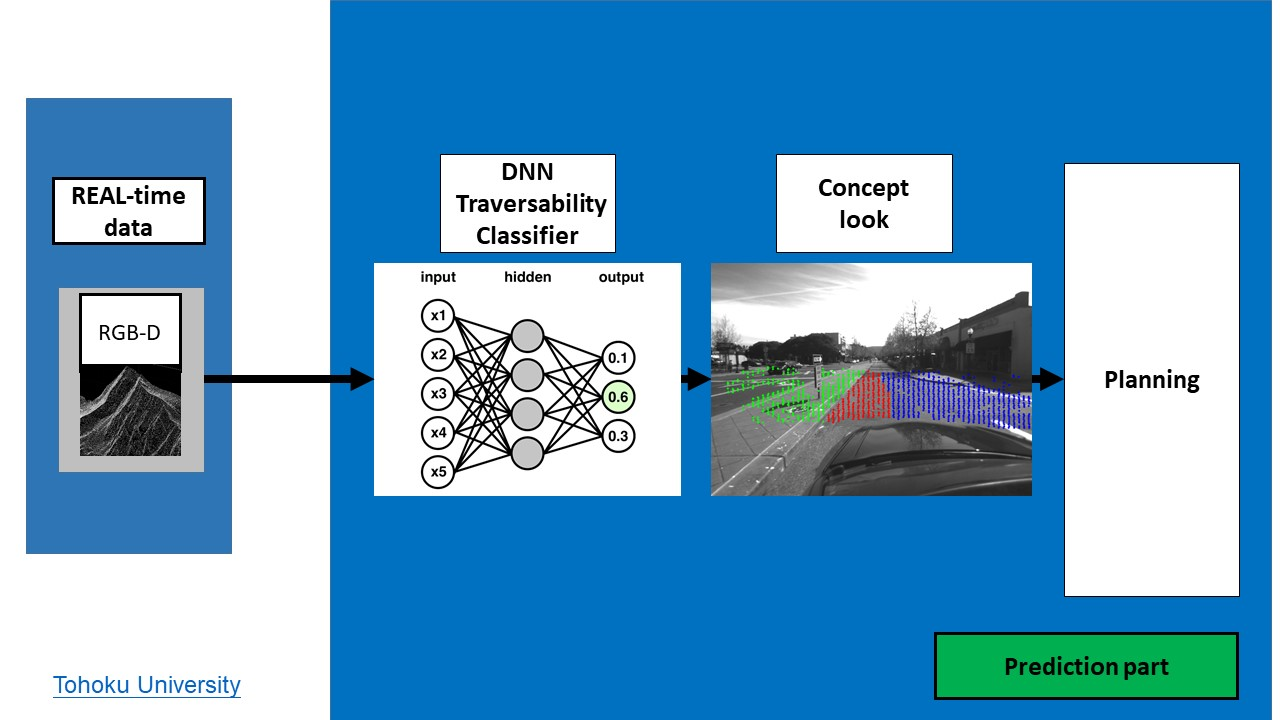
\includegraphics[width=0.8\columnwidth]{sys2}
\centering
\caption{Prediction}
 \label{figure:prediction}
\end{figure}




\section{SPECIFIC AIMS}

In our system, we want to use point cloud, robot model such as falling angle, mass, and inertia, and travesibility as the high-dimensional input of DNN. The output of DNN will be the ground truth of patches of the enviroment. In this part, I will explain the detail of point cloud and travesibility.
\begin{itemize}
\item Specific Aim 1 , Patches

Dividing the point cloud into patches, and do the simple corner detector. 
\item Specific Aim 2 , Travesibility

Robot can use travesibility to label every patches, and know the world frame of every patches
\end{itemize}

\section{APPROACH}
We will use VoxelGrid filter to downsample the point cloud, avoid many computing issue, and use transformation from the stereo camera frame to the odom frame to get the x,y,z of every pixel. After knowing the x,y,z of the pixel, we can divide the whole point cloud into many patches or superpixel \cite{kim2007traversability}, this will help thee robot tell the relative direction of different patches, and it will be used to do sample-based planning algorithm after giving the ground truth from the DNN model to every patch.

Travesibility will be computed using the algorithm from \cite{JiatongBao2012}, it will use a five dimensional vector (angular velocity of raw, pitch and linear acceleration of raw,pitch and yaw).
We will try different ways to compute travesibility in different ways because travesibility is objctive, and it will highly connected with the robot model, we will try the best algorithm in our scenario.

\section{SCHEDULE AND TEAM COLLABORATION}

Tommy Song : focusing on pcl processing and how to analyze imu data, different ways to calculate traversibility.

Lily Hsu : Robot Model, Terrain Model

Michael Tsai : DNN


  
\addtolength{\textheight}{-12cm}   % This command serves to balance the column lengths
                                  % on the last page of the document manually. It shortens
                                  % the textheight of the last page by a suitable amount.
                                  % This command does not take effect until the next page
                                  % so it should come on the page before the last. Make
                                  % sure that you do not shorten the textheight too much.

\bibliographystyle{IEEEtran}
\bibliography{egbib}

\end{document}
